\documentclass{article}
\usepackage{graphicx}
\usepackage{listings}
\usepackage{siunitx}
\usepackage{placeins}
\usepackage{amsmath}

\begin{document}

The application I thought of for multi-agent systems was Countries' GDP over time
as they interact with each other economically.
\\\\
To start our code generates a network graph for us using the adjacency matrix:
\[A =
\begin{bmatrix}
0 & 1 & 1 & 0 & 0 & 0 \\
1 & 0 & 1 & 0 & 0 & 0 \\
1 & 1 & 0 & 0 & 0 & 0 \\
0 & 0 & 0 & 0 & 1 & 1 \\
0 & 0 & 0 & 1 & 0 & 1 \\
0 & 0 & 0 & 1 & 1 & 0
\end{bmatrix}
\]
the weights would represent the amount of economic influence a country has on another but in our case we will leave them as 1 indicating that every country's influence is equal
\\\\
this generates our network graph as:
\begin{figure}[htbp]
    \centering
    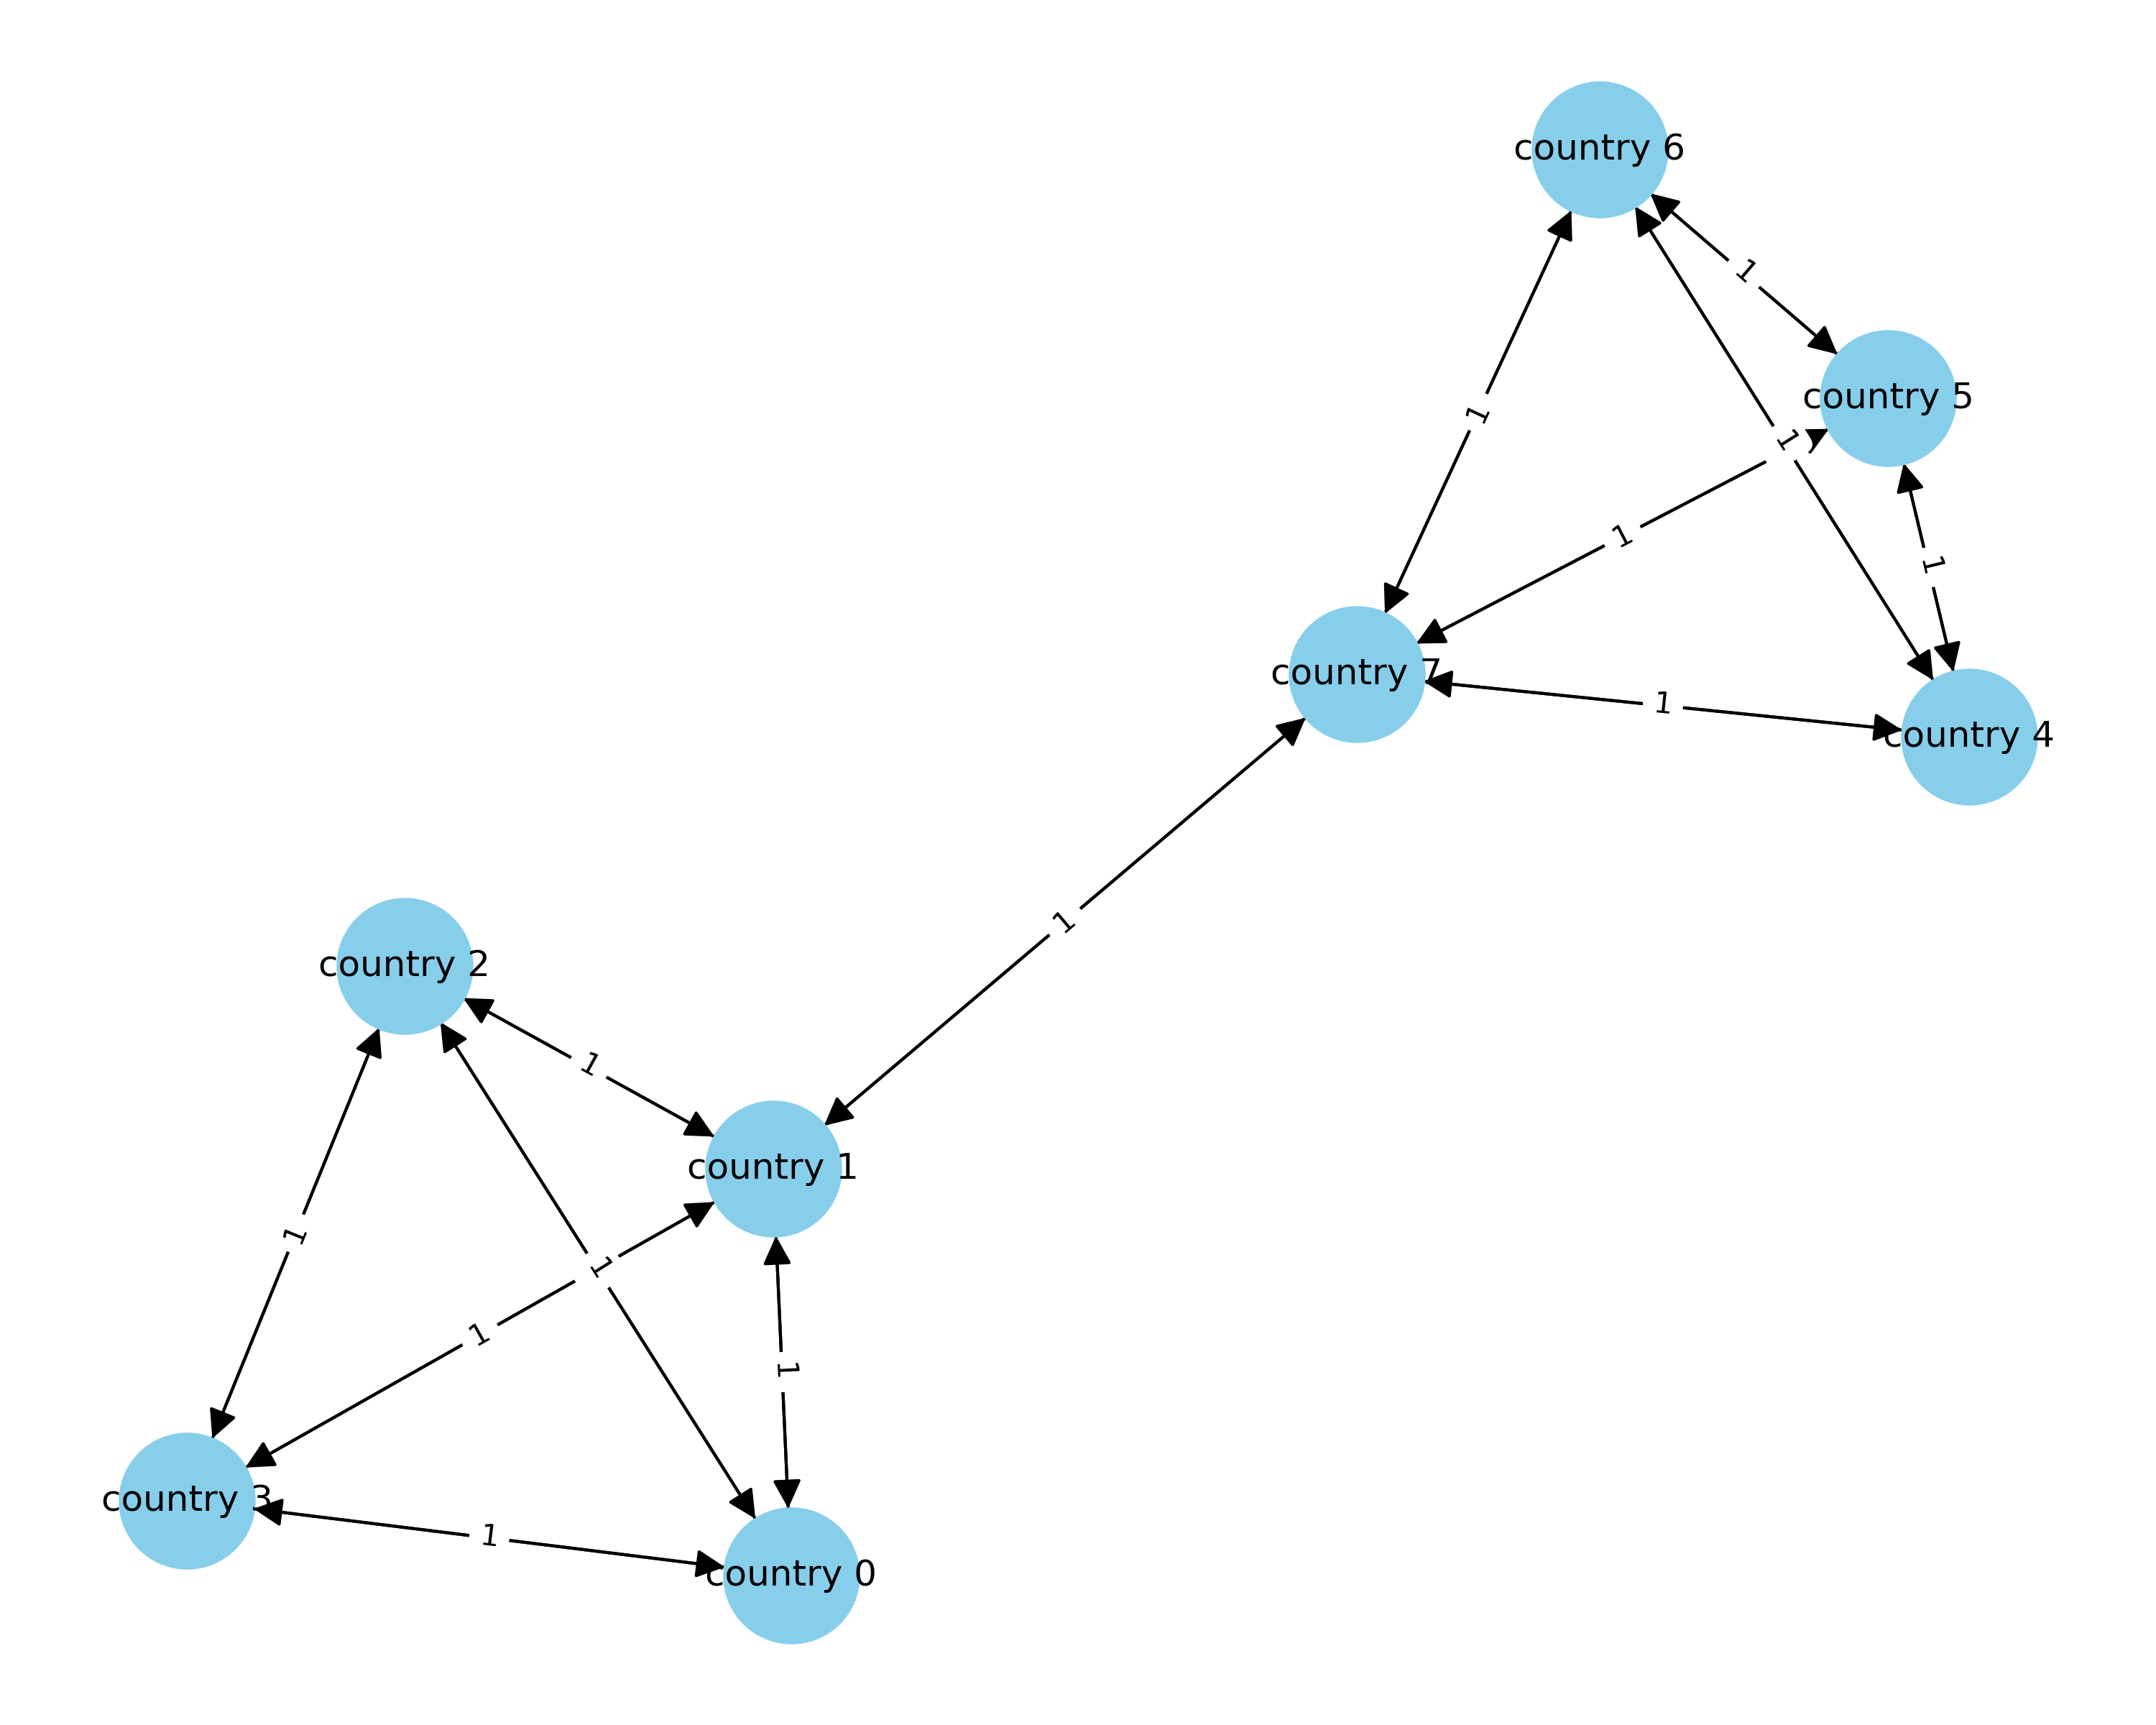
\includegraphics[width=0.8\textwidth]{directed_graph.png}
    \caption{network graph}
    \label{fig: directed_graph.png}
\end{figure}
\FloatBarrier

\newpage

from our network graph we can identify a set of differential equations that represent the combined effects on each country's GDP:

\[
\begin{aligned}
\frac{dC_0}{dt} & = 1(C_1 - C_0) + 1(C_2 - C_0) + 1(C_3 - C_0) \\[10pt]
\frac{dC_1}{dt} & = 1(C_0 - C_1) + 1(C_2 - C_1) + 1(C_3 - C_1) + 1(C_7 - C_1) \\[10pt]
\frac{dC_2}{dt} & = 1(C_0 - C_2) + 1(C_1 - C_2) + 1(C_3 - C_2) \\[10pt]
\frac{dC_3}{dt} & = 1(C_0 - C_3) + 1(C_1 - C_3) + 1(C_2 - C_3) \\[10pt]
\frac{dC_4}{dt} & = 1(C_5 - C_4) + 1(C_6 - C_4) + 1(C_7 - C_4) \\[10pt]
\frac{dC_5}{dt} & = 1(C_4 - C_5) + 1(C_6 - C_5) + 1(C_7 - C_5) \\[10pt]
\frac{dC_6}{dt} & = 1(C_4 - C_6) + 1(C_5 - C_6) + 1(C_7 - C_6) \\[10pt]
\frac{dC_7}{dt} & = 1(C_1 - C_7) + 1(C_4 - C_7) + 1(C_5 - C_7) + 1(C_6 - C_7)
\end{aligned}
\]
\noindent
We then put this into a vectorized equation to make it easier to work with:

\[
\frac{d\mathbf{C}}{dt} = -L \mathbf{C},
\]
or
\[
\frac{d}{dt}
\begin{bmatrix}
C_0 \\ 
C_1 \\ 
C_2 \\ 
C_3 \\ 
C_4 \\ 
C_5 \\ 
C_6 \\ 
C_7
\end{bmatrix}
\quad
=\ -
\begin{bmatrix}
 3 & -1 & -1 & -1 &  0 &  0 &  0 &  0 \\  
-1 &  4 & -1 & -1 &  0 &  0 &  0 & -1 \\  
-1 & -1 &  3 & -1 &  0 &  0 &  0 &  0 \\  
-1 & -1 & -1 &  3 &  0 &  0 &  0 &  0 \\  
 0 &  0 &  0 &  0 &  3 & -1 & -1 & -1 \\  
 0 &  0 &  0 &  0 & -1 &  3 & -1 & -1 \\  
 0 &  0 &  0 &  0 & -1 & -1 &  3 & -1 \\  
 0 & -1 &  0 &  0 & -1 & -1 & -1 &  4  
\end{bmatrix}.
\begin{bmatrix}
    C_0 \\ 
    C_1 \\ 
    C_2 \\ 
    C_3 \\ 
    C_4 \\ 
    C_5 \\ 
    C_6 \\ 
    C_7
\end{bmatrix}
\]

\newpage

this system can now very easily be solved numerically using a python package like \lstinline|scipy.integrate.solve_ivp|. First we must decide on an initial condition which will be GDP as a measure of economic strength in this case it has been randomly generated to be between 0 and 10 trillion and is given as the list 
\\$y_0$= [6.206, 8.651, 8.680, 4.312, 2.511, 4.770, 9.528, 4.389]

after solving the system we can then plot the solution over time to see how the GDP of each country changes over time:
\begin{figure}[htbp]
    \centering
    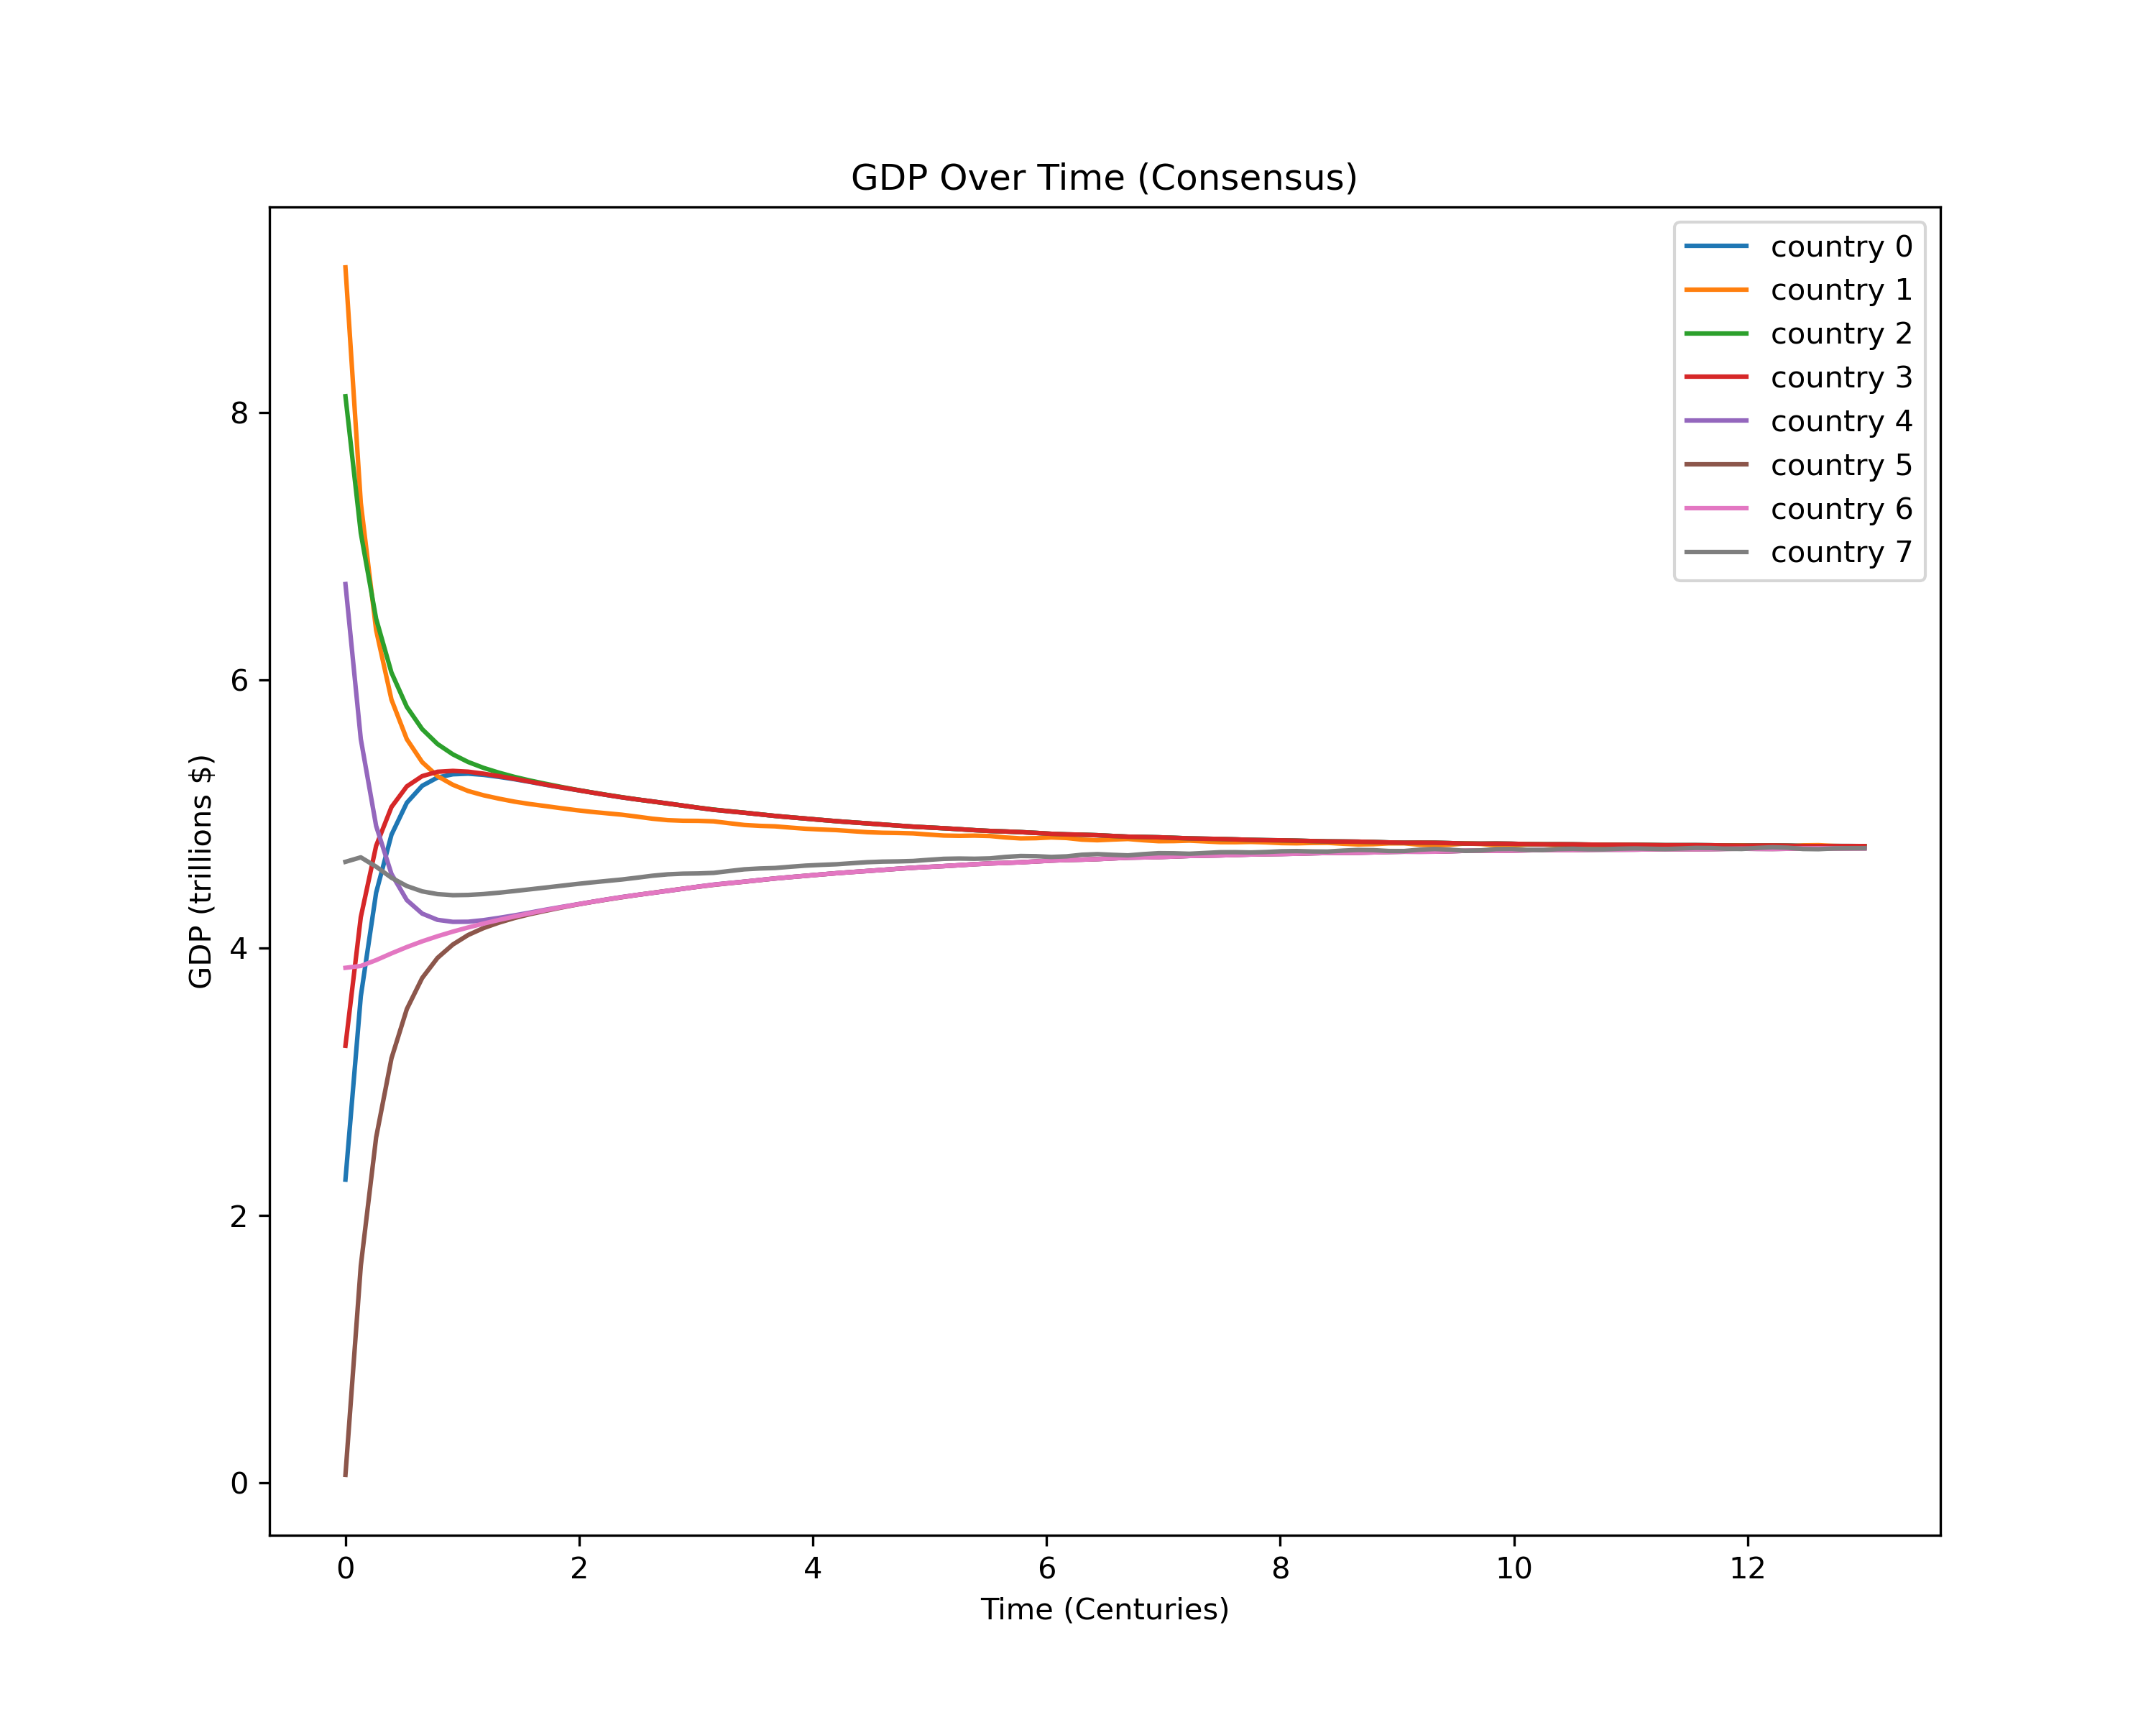
\includegraphics[width=0.8\textwidth]{consensus.png}
    \caption{GDP vs Time}
    \label{fig: consensus.png}
\end{figure}
\FloatBarrier
\noindent
As we can see the countries change their GDP rapidly at first before eventually reaching consensus around GDP = \$4.756 trillion.

In practice we couldn't set the weights to 1 and would have to set them to be a function of the amount of economic influence a country has on another country with respect to time, which would make our calculations more complex. but this shows how globally we might trend towards a consensus point where global GDP per capita is the same as the GDP per capita in each country. Another insight we can infer from the directed graph is that this consensus occurs even when there are distinct economical systems with only minimal effects between them


\end{document}